\section{3.9 Efekt Rungego}
\begin{frame}
{3.9 Efekt Rungego}

(C. Runge, 1901)
$$
y(x)=\frac{1}{1+25x^{2}},\ x\in[-1,\ 1]
$$
Występuje, gdy:
\begin{itemize}
\item wielomiany

\item równoodległe węzły
\end{itemize}

Rada praktyczna:

\begin{itemize}
\item zaczynać od interpolacji liniowej,

\item zwiększać liczbę węzłów i stopień wielomianu aż do ustabilizowania istotnych miejsc.
\end{itemize}


Sposób $\rightarrow$ \textbf{interpolacja przedziałowa}.
\begin{itemize}
\item katastrofalna rozbiezność dla $0.726\leq|x|<1$

\item b. dobra zbieżność w strefie centralnej
\end{itemize}

(konsekwencja tego, że zadanie to jest {\itźle uwarunkowane})
\end{frame}
\begin{frame}
\begin{figure}[h]
			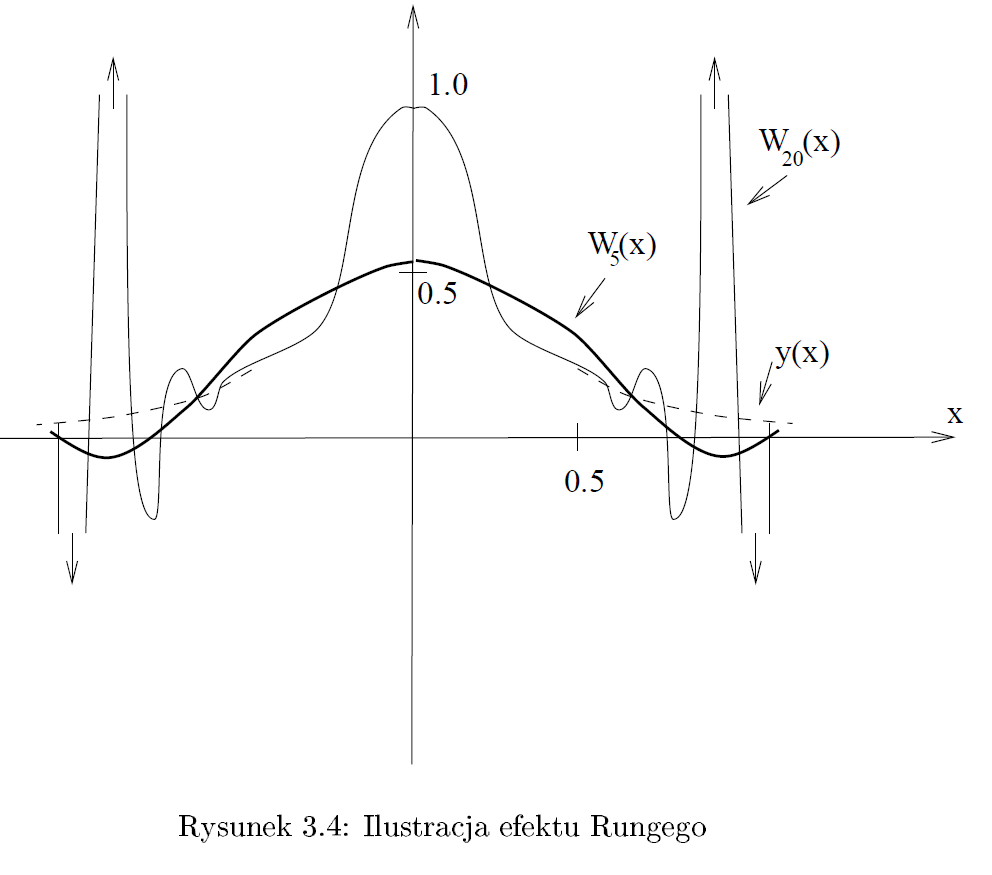
\includegraphics[scale=0.35]{img/3/interpol_3_9}
	\end{figure}
\end{frame}